\documentclass[10pt]{article}
\usepackage{srcltx,graphicx}

\textwidth 6 in \textheight 8.75 in

\voffset-.75in \oddsidemargin.25in \evensidemargin.25in

\begin{document}

\begin{center}
 {\huge \bf Riverside Research Institute}
\end{center}

{\bf To:} Users of new data acquisition system

{\bf From:} Jeff Ketterling

{\bf Date:} \today

{\bf Subject:} How to use LabVIEW based software for acquiring RF
data.
\\

This memo discusses the operation of the LabVIEW software used to
acquire RF data from a Hitachi, B\&K 3535, or Hawk ultrasound
scanner. A brief overview of the hardware, wiring connections, and
installed software is also included. The LabVIEW software permits
the acquisition, viewing, and saving to disk of a collection of
scans. The data can be viewed as individual files or as a
collection of thumbnails. The data is saved to disk in the RRI EYE
file format.
%\\ \hline

\section{Hardware}

\subsection{Wiring Overview}

The operation of the software requires the installation of two PCI
cards in the host computer. These are a GaGe 12100 50 Ms/S 12 bit
A/D card and a National Instruments PCI6601 counter/timer card.
The GaGe card allows for RF data acquisition and the 6601 card
permits proper triggering so data acquisition begins at the start
of a video frame. In addition to the two PCI cards a small break
out box is needed to properly route the signals between the
ultrasound scanner and the host computer.

The wiring connections are shown in Fig.~\ref{fig:wiring}. Both a
frame sync and vector sync line go from the Hitachi and Hawk (only
vector sync if using a B\&K 3535) to the break out box. The
trigger output from the break out box and the RF line from the
Hitachi and Hawk go to the GaGe PCI card in the host computer. A
B\&K 3535 system has no frame sync and also has a TGC line going
to CH.~B of the GaGe board. The B\&K Hawk system has a 40 MHz
sample clock line. Finally, a ribbon cable from the 6601 card
connects to the break out box.

\begin{figure}[htb]
\begin{center}
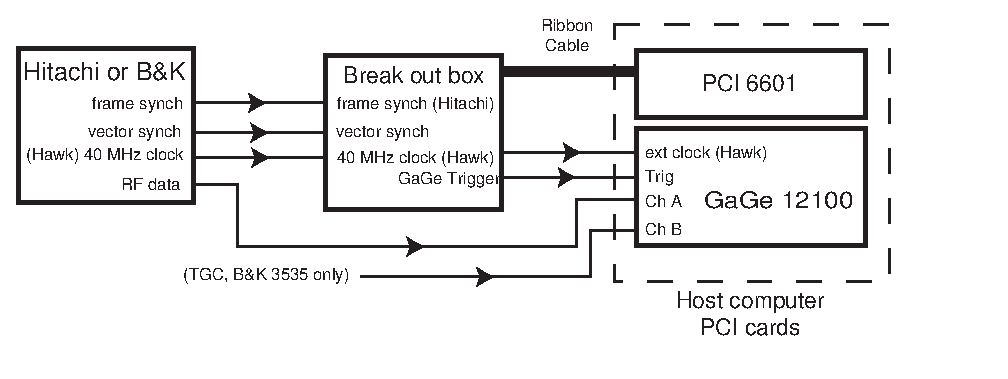
\includegraphics[width=4.2 in]{wiring.eps}
 \caption{Wiring diagram for equipment using Hitachi and Hawk systems. Note
 that for a B\&K 3535 system, wiring is identical except there is no frame
sync line. The Hawk system has a 40 MHz sample clock.}
 \label{fig:wiring}
\end{center}
\end{figure}

\subsection{Operational Overview}

The 6601 PCI card provides the key to the data acquisition system
by allowing data to be taken at the start of a video frame. This
is accomplished using a single counter for the Hitachi and the
Hawk. The counter is armed via a hardware trigger when the frame
sync goes from high to low. The counter then generates a single
output pulse every time the vector sync goes from high to low.

Triggering for the B\&K 3535 is similar except that a second
counter is used to generate a frame sync pulse. This is necessary
because the B\&K does not provide a frame sync. The frame sync is
created by taking advantage of the fact that the the vector sync
pulses for a single frame are separated by some ``dead'' time. The
duration of the dead time is just under 28 ms when the B\&K is
operated at 10 frames/s and a resolution of 6. By generating a
non-resettable 75 ms pulse on the falling edge of the vector sync
signals, a frame sync can be created that lines up with the first
vector after several video frames have passed.

The 6601 PCI card also allows for triggering on a single vector
sync to assist in probe calibration. This is done by using a
single counter. The frame sync triggers the counter and then the
edges of the vector sync are counted on the counter's source to
generate a delayed pulse. For example, to extract the 5th vector,
five falling edges are counted on the source before an output
pulse is generated. One output pulse is generated for every frame
and thus only one RF scan line is captured for each frame.

The triggers generated by the 6601 initiate data acquisition on
the GaGe 12100. When a scan is taken, the GaGe acquires the full
number of vectors (scan lines) for a single video frame, and then
the data is transferred to the host computer. The data is
available for viewing until saved and deleted.

Note that for the B\&K 3535, TGC data can also be taken on Ch.~B
of the GaGe card. Thus, the GaGe board may require a deeper memory
for a B\&K 3535. The GaGe board operates in dual channel mode for
a B\&K, while the Hitachi operates in single channel mode.
However, if a rapid series of frames needs to be captured, the
B\&K TGC signal can be ignored and the GaGe board operated in
single channel mode. The amount of memory available on the GaGe
board determines how many consecutive frames of video can be
captured.

\section{Software}

\subsection{Clinical Version} The software will already be
installed on the host computer in most circumstances. This section
is meant more as a reminder of what to install if starting a new
system from scratch. The actual working piece of software will
normally be a Run-Time only LabVIEW application named
GetProstateData. The run-time engine version of LabVIEW 6i needs
to be installed on the host computer in order to run the software.
The files daqdrv, lvanlys.dll, lvdaq.dll, and serpdrv need to be
in a folder named {\it data} in the same directory as
GetProstateData. NI-DAQ, which contains the drivers for the 6601
card, and GaGe drivers also need to be installed.

\subsection{Research Version}

The research version of the software permits calibration data to
be taken, allows modification of low level parameters, and
provides a few additional features. If the software is a Run-Time
only version, than no additional software is needed. However, if
it is the full, modifiable code, LabView 6.1 is needed. In
addition, all relevant VI libraries must be present on the host
computer.

\section{Using Software to Acquire data}

\subsection{Features in Clinical Version}

The operation of the data acquisition software GetProstateData is
straightforward and uses controls that are familiar from commonly
used software applications. The software is executed by double
clicking the application GetProstateData. A shortcut will normally
be on the desktop and in the Windows Start menu. When the
application is executed, a window opens (Fig.~\ref{fig:getdata})
with the software already running.

\begin{figure}[htb]
\begin{center}
\includegraphics[width=5.8 in]{getdata.eps}
 \caption{User interface of GetProstateData.}
 \label{fig:getdata}
\end{center}
\end{figure}

Before taking new data, enter the parameters for {\it Patient
Info, Operator Initials}, and {\it Transducer ID}. These
parameters will be placed in the saved EYE files. {\it RRI ID} is
limited to 6 characters and will form the base name of all the
saved files. {\it Hospital ID} is limited to 10 characters and
operator initials to 4 characters.

Next select the appropriate system and probe from the pull down
menu at the bottom of the screen. The probe can be changed without
stopping the program. Be careful not to select the Hawk settings
unless a Hawk system is being used. If the 40 MHz sample clock is
not plugged into the GaGe card on a Hawk system, the software will
freeze and will need to be restarted. If the Multiframe option is
selected, a number will appear listing the total number of
consecutive frames that will be acquired upon each scan.

Data is acquired by pressing {\bf Start Scan} or pushing the {\bf
F1} key. Once acquired, the data will appear in the plot window of
Fig.~\ref{fig:getdata} and the computer will beep. {\bf A color of
red in the plot means the digitizer was saturated. Choose a lower
value for {\it Gage Sens} until no red is visible.} Each time a
new scan is captured with GetProstateData, the display is updated.
To view a previous scan, go to the {\it Scan to View} Control,
select it by clicking on it with the mouse, and choose the file
you want to view (Fig.~\ref{fig:case}). The switch next to the
name of the case being viewed
\includegraphics[width=0.4 in]{keep.eps} indicates whether or not the data will
be saved. {\bf If no data is received, an error message will be
displayed. Erase all the data if no scans prior to the error need
to be saved.}

\begin{figure}[htb]
\begin{center}
\includegraphics[width=1.5 in]{case.eps}
 \caption{Select case to view by using pop up menu.}
 \label{fig:case}
\end{center}
\end{figure}

Selecting {\it View Thumbnails} will show small thumbnail images
of the acquired scans with the file name overlaid on the image.
The images are in sector format. Once all data has been acquired,
select {\it Save All Data} to save the data as EYE files. A dialog
will inform the user that all the data has been saved and that it
is now safe to delete it from temporary memory. Then select {\it
Erase All Data} to delete all of the data and start a new data
acquisition. Another dialog will prompt the user to confirm that
the data should really be erased.

To exit the program select {\it Done}. A prompt will check to see
if the user really wants to quit and then another prompt will ask
if the data should be sent to RRI via FTP. A window will indicate
that an FTP operation is in progress. An email will also be sent
to RRI to indicate data has been transferred. Once data has been
sent via FTP it will be moved to a folder named Previous Scans on
D:$\backslash$ and the GetProstateData program will close
automatically. Data that has not yet been sent or that has just
been captured is saved in a folder named Current Scans on
D:$\backslash$. {\bf If a problem occurs during the FTP process,
the program may crash but the data will not be deleted. It will be
sent the next time FTP and Quit is selected.} If no FTP option is
available in the software, data will need to be copied either
manually or with a separate application (described below) to a Zip
disk.

Two features are included to modify how the data is viewed in the
display window. These buttons are located below the display. {\it
Axis as count} can be altered to {\it Axis as range}, changing the
axis hash marks to a range in mm. This is meant to allow features
of the image to be related to a distance. The other option, {\it
Linear Grey Scale} or {\it Log Grey Scale}, changes the display
mapping to show less or more contrast. Neither setting effects the
data acquisition or how data is saved to EYE files.

An option may also be present to take a series of consecutive
frames. If so, the number of frames is determined by the depth of
GaGe memory and how much data is in each frame. The data is
acquired as described above. All the frames are viewable as
thumbnails but only the first frame is displayed in
Fig.~\ref{fig:getdata}. The file naming convention takes the RRI
ID and appends the scan number followed by a letter a and then a
number for each consecutive frame. For example, if the RRI ID is
Q22r and there are 4 consecutive frames per scan, then the naming
would be Q22r1a1, Q22r1a2, etc.~for the first scan and Q22r2a1
etc.~for the second scan. The thumbnail images will show all of
the captured data and have the proper file name overlaid.

\subsection{Features in Research Version}

The research version of the software looks just like
Fig.~\ref{fig:getdata} except two additional features are added.
One allows the low level settings of the digitizer to be modified.
This feature is essential when first setting up a system to ensure
that all the default parameters for later use are properly chosen.
The low level parameters are accessed via a control panel that
looks much like an oscilloscope. A control selects which vector
line to view and the RF data from this line is displayed as an RF
trace.

The other option of the Research Version allows data to be taken
either as a single frame or a single vector. The single vector
setting is meant to acquire calibration files as an image with the
same vector line taken over multiple frames.

\subsection{Saving data to Zip disk}

A small LabView application named SaveToZip will also have a short
cut on the desktop to streamline the process of copying files to a
Zip disk and and moving files from the Current Scans folder to the
Previous Scans folder. When the application is run, a window will
open indicating that files are being copied to the Zip disk. Two
possible warnings may arise: one if no Zip disk is present in the
Zip drive, and one if the Zip disk cannot hold all of the new
files being copied. If a warning is given, press OK, and run the
program again after taking the appropriate corrective action. When
SaveToZip has run successfully, an email will automatically be
sent to RRI indicating data has been captured.
 {\bf Make sure the Zip drive light is off before ejecting the
Zip disc. Files may still be copying, even if the SaveToZip
program has closed.}

\subsection{FTP data to Riverside}

A separate LabView application named FTPAllData may be available
to FTP data to Riverside after data has been acquired. The
computer needs to be connected to the internet first. Once the
application is run, the computer can be left alone and all the
data will be automatically transferred to RRI. An email message
will be sent confirming the transfer of data. The email will list
the filenames that were transferred and any errors that may have
occurred.

\pagebreak \clearpage

\subsection*{{\Large Simple overview of LabVIEW data acquisition software}}

\begin{enumerate}
\item Double click {\bf GetProstateData} on the desktop to start the RF data acquisition application.
The application user interface (pictured below) will open and
start running.

\item Select appropriate probe from pull down menu at bottom of
screen.

\item Select {\it Multiframe} option if acquiring a sequence of
consecutive frames.

\item Enter parameters in the {\it Patient Info} box.

\item Push {\it Take Scan} or {\it F1} when ready to take data.
A beep will indicate when the data has been acquired. If red
appears in the image, lower {\it Gage Sens}, {\it Clear All Data}
and take another scan. (A small amount of red may be acceptable.)

\item Take as many scans as needed. Or take test scans, and then select
{\it Clear All Data} before taking final data that will be saved.

\item Previous scans can be viewed by using the {\it Scan to View}
control. All of the scans can be viewed as thumbnails by selecting
{\it View Thumbnails}.

\item Scans that do not need to be saved can be excluded by
choosing {\it Discard} next to the scan number shown in the {\it
Scan to View} control.

\item When ready to save data, select {\it Save All Data}. A
prompt will indicate when data is saved.

\item The data can now be cleared by pushing {\it Clear All Data}.
A prompt will ensure that the data should really be deleted. A new
{\it RRI ID} can now be entered and more data taken.

\item To exit the program, select {\it Done}. A window will open asking
whether to really quit. An option may also be present for quiting
and FTPing data to RRI. If data can be FTPed, a window will open
while data is being sent to RRI. If not, the program will close.

\item Newly acquired data is stored in a folder called Current
Scans on D:$\backslash$.~If data is FTPed successfully to RRI it
will be transferred to a folder named Previous Scans on
D:$\backslash$. If no FTP option is available, the data in the
Current Scans folder should be transferred to a Zip disk and the
Previous Scans folder with the {\bf SaveToZip} application on the
desktop. Zip disks should then be sent to RRI.

\end{enumerate}

\begin{figure}[b]
\begin{center}
\includegraphics[width=3.1 in]{getdata.eps}
\end{center}
\end{figure}


\end{document}
